\section{Southern Ocean extrapolation}
  \label{sup:sec:SOExtrapolation}

  \subsection{Outline}
    We use simulated tropospheric ozone columns from GEOS-Chem to extrapolate the ozonesonde-based estimates to the entire Southern Ocean region, defined here as 35$^{\circ}$ S-75$^{\circ}$ S to encompass our three measurement sites. 
    To determine the ozone column attributable to STT, we determine monthly averaged STT impact (\textit{I}) and the monthly mean tropospheric ozone column over the Southern Ocean (from the GEOS-Chem multi-year mean, $\Omega_{SO_{O_3}}$), expressed simply as flux$_{per event} = \Omega_{SO_{O_3}} \times I$.
    This value gives us the STT flux per event in each month.
    Next we determine how many events are occuring per month, using a few of assumptions: we assume only one event can occur at one time, and that no event is measured twice.
    These assumptions are not realistic, however they allow a simple estimate of events per month from the relatively sparse dataset.
    The monthly likelihoods of STT is calculated from fraction of ozonesonde releases for which an STT event was detected, within each month, \textit{L}.
    And if we assume events last N days, we find how many events per month by multiplying the days in a month by L and dividing by the assumed event lifetime.
    For example if we expect to see an event 25\% of the time in a month, and events last one day, we expect one event every four days ($\sim 7.5$ events in that month) whereas if we expect events to last a whole week then we would expect $\sim$one event in that month.
    This leads us to multiply our flux$_{per event}$ by L, and then by the range dictated by our assumed event lifetime.
    
    Figure \ref{sup:fig:SOExtrapolation} (upper panel) shows the factors I, L, and $\Omega_{SO_{O_3}}$ which are used along with the assumed event lifetime to estimate the STT flux.
    The tropospheric ozone and area of our region is calculated using the output and surface area from GEOS-Chem over the Southern Ocean grid boxes along with the molecules cm$^{-2}$ per month calculations, along with ozone molar mass of 48~g mol$^{-1}$.
    
    It is worth noting that this extrapolation is very simplistic and is performed as an example of how the seasonal ozone STT calculations could be used.
    A more spatially resolved estimate could be determined by dividing the Southern Ocean region into longitudinal and latitudinal bins for calculating the average $\Omega_{SO_{O_3}}$ from GEOS-Chem, applying latitudinal gradients to $L$ and $I$ based on their values at the three sonde release sites, and adding longitudinal variability due to seasonal stratospheric wind jet streams \citep{Baray2012,Skerlak2015}.
    An improved estimate of event lifetime and parameterisation of how many events may be occuring simultaneously could also be addressed, however this is beyond the scope of this work and in any case would not address all the limitations of the estimate provided below.
    %  This result highlights the difficulty associated with extrapolating from temporally sparse ozonesonde data, as STT impact is hard to measure without multiple measurements during and surrounding each event.
  \subsection{Results}
    
    Fig. \ref{sup:fig:SOExtrapolation} (lower panel) shows the results of the calculation when we choose 2.5 days for our flux estimation, with the range shown in representing the values calculated if we assume events last 1 day (upper bound of estimated flux) or one week (lower bound of estimated flux).
    Previous studies have found STT ozone fluxes in the SH extratropics are largest from autumn or winter to early spring \citep{Olsen2003, Liu2016}.
    At this time of year, we find the highest tropospheric $\Omega_{O3}$ but a relatively low STT flux due to reduced event frequency.
    Our results suggest instead that the ozone flux associated with STT events (at least those due to tropopause folds) is largest in austral summer (December-March), primarily due to an increased frequency of STT detections during these months.
    It is possible that our estimated event frequencies are too low in late winter-early spring as some legitimate STT events may have been excluded due to coincident smoke plumes.
    
    \begin{figure}[t]
      % Plot from examine_stations.py in stations repo
      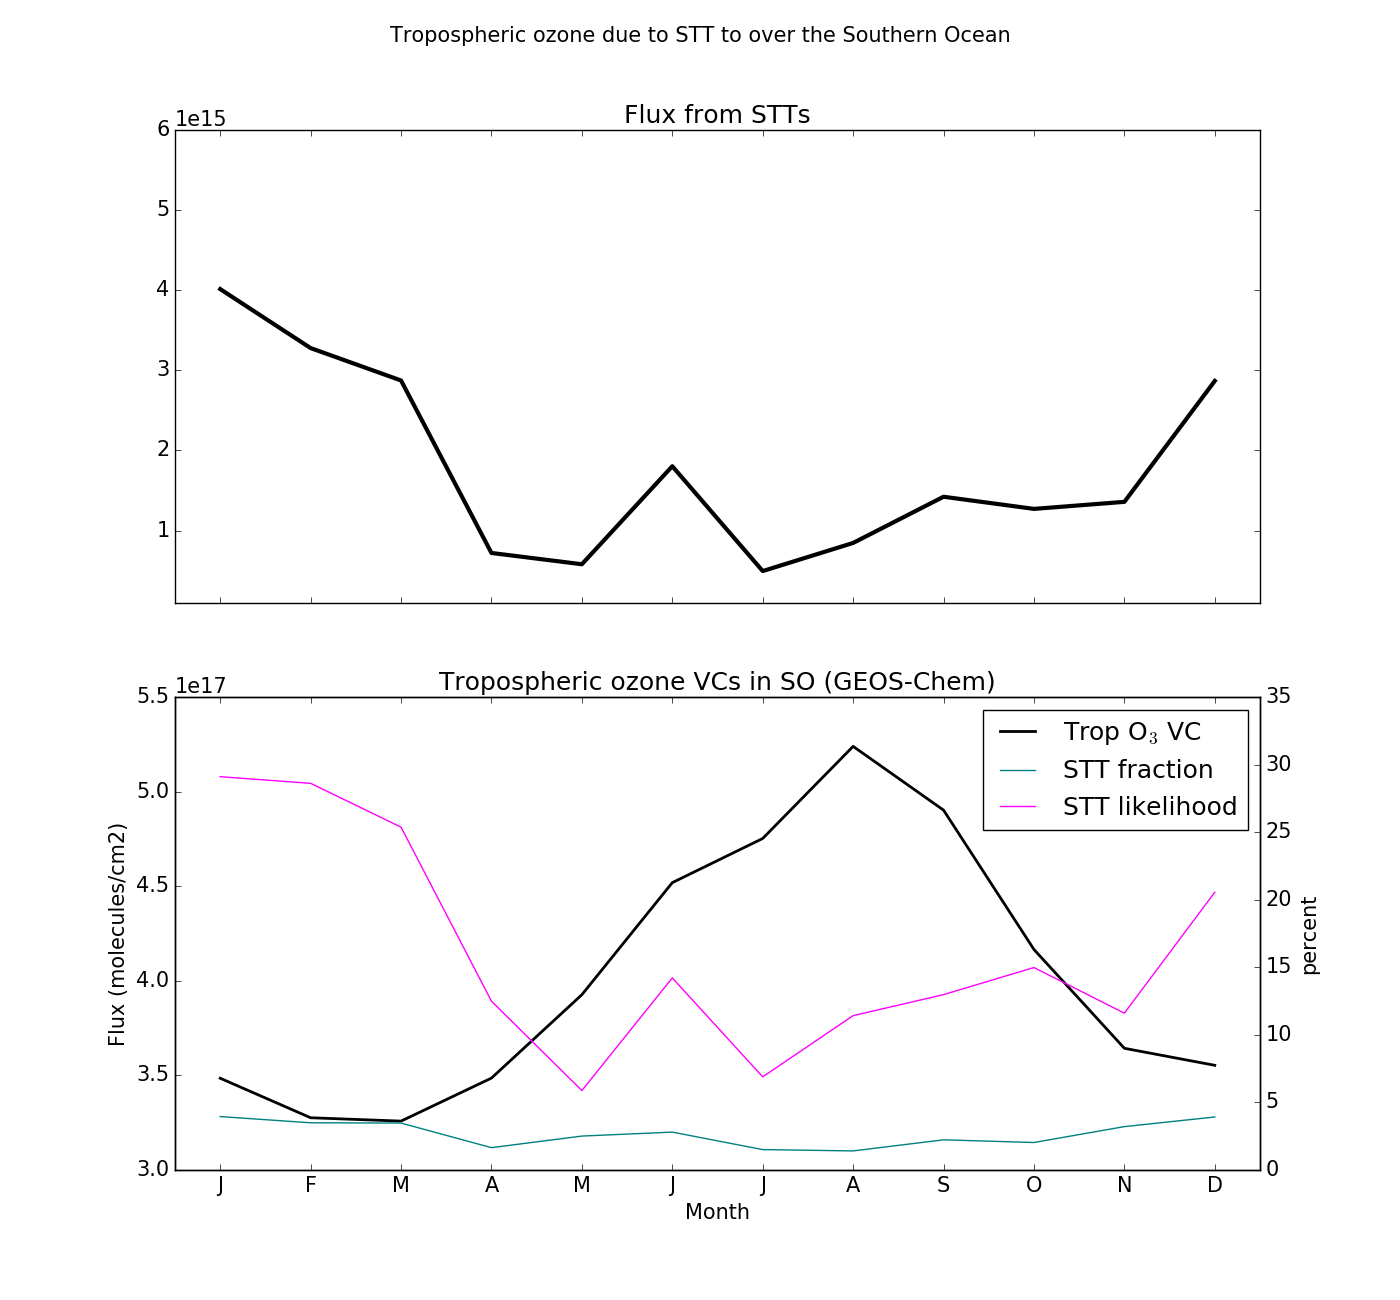
\includegraphics[width=12.0cm]{../figures/SO_extrapolation.png}
      \caption{%
	(Top) The three quantities used to calculate the total Southern Ocean ozone flux from STT events.
	The tropospheric ozone column $\Omega_{SO_{O_3}}$ (black, left axis) is from GEOS-Chem, while the STT fraction $f$ (magenta, right axis) and Impact $I$ (teal, right axis) are from the ozonesonde measurements.
	The STT impact is multiplied by 3 to better show the seasonality.
	(Bottom) Estimated contribution of STT to tropospheric ozone columns over the Southern Ocean.}
      \label{sup:fig:SOExtrapolation}
    \end{figure}
    
    Summing the monthly estimated fluxes shown in Fig. \ref{sup:fig:SOExtrapolation} over the year, we find from this estimate that STT events may be responsible for at least $3.1 \times10^{16}$~molecules cm$^{-2}$ yr$^{-1}$ of the tropospheric ozone over the Southern Ocean, equivalent to 2.48~Tg yr$^{-1}$.
    $1$-$6 \times 10^{16}$ molecules cm$^{-2}$ of stratospheric based ozone is estimated over the southern ocean throughout the year.
    Our estimate is smaller than expected from prior work that suggests global gross STT fluxes of 550~Tg yr$^{-1}$ \citep{Stevenson2006} and net downward STT fluxes of 75~Tg yr$^{-1}$ \citep{Sprenger2003}.
    Our value would suggest only $\sim$3.3\% of this global net downward flux can be attributed to STT events in the Southern Ocean region, a contribution that is likely too low.
    This result is only marginally sensitive to the latitude range chosen to represent the Southern Ocean (35$^{\circ}$ S-75$^{\circ}$ S): changing this range by 5$^{\circ}$ in either direction at either end of the range changes $\Omega_{SO_{O_3}}$ by -7 to +9\%, with even smaller impacts on the overall flux.
    
    %Our estimate is smaller than other estimates of STT flux, due to our conservative estimate of flux within each event, as well as filtering out events which are too close to the tropopause.
    %Global STT flux estimated from an ensemble of models suggests values around 550~Tg yr$^{-1}$ \citep{Stevenson2006}.
    %Global net downward STT flux is estimated to be 75~Tg yr$^{-1}$ \citep{Sprenger2003}.
    %Previous studies have derived global gross STT fluxes of 550~Tg yr$^{-1}$ \citep{Stevenson2006} and net downward STT fluxes of 75~Tg yr$^{-1}$ \citep{Sprenger2003}.
    %Our estimate of 2.48~Tg yr$^{-1}$ would suggest only $\sim$3.3\% of the global net downward flux can be attributed to STT events in the Southern Ocean region, a value that is likely too low.
    %This method of flux estimation could be increased if we could account for background ozone enhancement and mixing due to events.
    
    If we we assume a fractional ozone impact due to each event STT event of $I$=35\% (rather than our calculation of $I$=2-4\%), our estimate of the net downward ozone STT flux from Southern Ocean STT events increases by an order of magnitude to $\sim$29.5~Tg yr$^{-1}$, equivalent to 39\% of the global net downward flux estimated by \citet{Sprenger2003}.
    The annual tropospheric ozone flux over the Southern Ocean due to STT events is $\sim3.2\times10^{16}$ molecules cm$^{-2}$ yr$^{-1}$.
    
    % From Abstract:
    %A conservative estimate of yearly tropospheric ozone flux due to STTs is calculated using the simulated tropospheric ozone column between 35$^\circ$ S and 75$^\circ$ S of $3.2\times10^{16}$ molecules cm$^{-2}$ yr$^{-1}$.
    %This value is significantly lower than expected from previous global estimates due to the conservative nature of several components of our calculation, in particular the contribution of STT to total tropospheric ozone during an event (STT impact).
    %Using an assumed STT impact of 35\% based on prior modelling studies rather than our observational estimate of 2--4\% increases the estimated Southern Ocean flux by an order of magnitude.%to $\sim$29.5~Tg yr$^{-1}$.
    %Despite lingering uncertainties in scaling ozonesonde measurements to regional values, ozonesonde datasets provide a useful tool for STT detection, and the analysis methods described in this paper could be applied to many existing long-term records.

\section{Fast fourier transform code (IDL)}
\label{sup:sec:FFTCode}
  Provided by Dr. Simon Alexander.
  
  \verbatiminput{sa_filter_1d.pro}